\documentclass[11pt]{article}

\usepackage[pdftex]{graphicx}
\usepackage{xcolor}
\usepackage{amsmath,amssymb,amstext,amsthm,standalone,tikz}
\usepackage{geometry}
\usepackage{fancyhdr}
\usepackage[pdftex]{graphicx}
\usepackage{xcolor}

\geometry{
  verbose,
  dvips,
  width=430pt, marginparsep=0pt, marginparwidth=0pt,
  top=90pt, headheight=12pt, headsep=20pt, footskip=30pt, bottom=80pt}

\setlength{\parskip}{\medskipamount}
\setlength{\parindent}{0pt}

\linespread{1.05}

\newtheorem{theorem}{Theorem}
\newtheorem{lemma}[theorem]{Lemma}
\newtheorem{proposition}[theorem]{Proposition}
\newtheorem{corollary}[theorem]{Corollary}
\newtheorem{conjecture}[theorem]{Conjecture}
\newtheorem{obs}{Observation}
\newtheorem{clm}{Claim}
\newtheorem{ques}{Question}
\newtheorem{problem}{Problem}

\newtheorem{ex}{Example}


\newcommand{\spc}{\hspace{0.08in}}
\newcommand{\vs}{\vspace*{.1in}}
\newcommand{\E}{\mathbb{E}}
\newcommand{\Prob}{\mathbb{P}}
\newcommand{\edit}[1]{\emph{\textcolor{blue}{#1}}}


\renewenvironment{proof}{{\noindent \textbf{\textit{Proof.}}}}
{\hfill $\Box$ \vspace*{0.1in}}
\newenvironment{proofc}{{\noindent \textit{Proof of Claim.}}}
{\hfill $\Box$}


\begin{document}
\begin{huge}
    \begin{center}
        Test 3 Review
    \end{center}
\end{huge}


\vs\vs

***Disclaimer*** Making up integration problems can be difficult since it is often deceivingly difficult to integrate simple surfaces. So I highly recommend using in-class examples (especially ones worked in the video recordings) along with this review to aid in studying.

\section{Prior to integrating}

\begin{problem}
    Rewrite the following expressions and equations in polar coordinates and graph the first two.
    \begin{enumerate}
        \item $2x^2 + 2y^2 = 19$
        \item $x^2+y^2 = 4x+6y$
        \item $\frac{\sqrt{x^2+y^2}}{xy}$
    \end{enumerate}
\end{problem}

\begin{problem}
    Rewrite the following in spherical coordinates and graph it.

\[x^2+y^2+z^2 = 10y\]

\end{problem}






\begin{problem}
Estimate the volume of the surface $f(x,y) = xy-(x+y)^2$ bounded by the region $R = \{(x,y): 1\leq x\leq 5, 0\leq y\leq 3\}$ with $n = 2$, $m=2$ ($n$ across the $x$-axis,$m$ across the $y$-axis) and 
\begin{enumerate}
    \item Lower left corner 
    \item midpoint
    \item upper right corner
\end{enumerate}
\end{problem}

\section{Multiple Integrals Set-up}
For each of the following problems, set up \emph{but do not evaluate} an expression using integrals which solves the given problem.

\begin{problem}
    The volume under the surface $f(x,y) = e^{\sin{xy}}$ bounded by $y = 3x-3$ and $y = x^2-3x+2$
\end{problem}

\begin{problem}
    The volume of under the surface $f(x,y) = \frac{x}{y}$ bounded by the region $x^2+y^2 =4x$ and $y=x$.
\end{problem}

\begin{problem}
The volume between $z = x^2y^3$ and $z=1$ and above the region $x^2+y^2 \leq 7$ 
\end{problem}

\begin{problem}
    The area of the following hexagon. 
    \begin{center}
    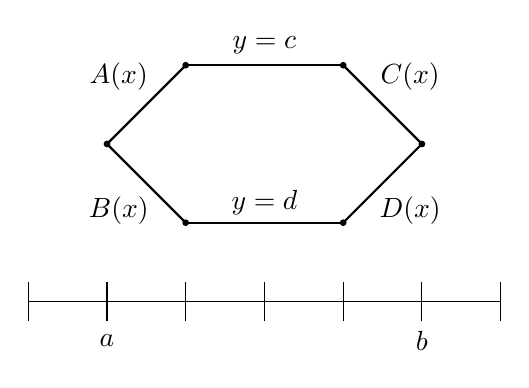
\begin{tikzpicture}


\draw[thick] (0,0) -- (2,0);
\draw[thick] (0,2) -- (2,2);
\draw[thick] (-1,1)--(0,2);
\draw[thick] (-1,1)--(0,0);
\draw[thick] (3,1)--(2,2);
\draw[thick] (3,1)--(2,0);


\draw (-2,-1) -- (4,-1);
\draw (-2,-1.25) -- (-2,-.75);
\draw (-1,-1.25) -- (-1,-.75);
\draw (0,-1.25) -- (0,-.75);
\draw (1,-1.25) -- (1,-.75);
\draw (2,-1.25) -- (2,-.75);
\draw (3,-1.25) -- (3,-.75);
\draw (4,-1.25) -- (4,-.75);




\draw[fill=black] (-1,1) circle 
(1pt);
\draw[fill=black] (0,0) circle (1pt);
\draw[fill=black] (0,2) circle (1pt);
\draw[fill=black] (2,0) circle (1pt);
\draw[fill=black] (2,2) circle (1pt);
\draw[fill=black] (3,1) circle (1pt);


\node at (-.85,1.85) {$A(x)$};
\node at (-.85,.15) {$B(x)$};
\node at (2.85,1.85) {$C(x)$};
\node at (2.85,.15) {$D(x)$};

\node at (1,2.25) {$y=c$};
\node at (1,0.25) {$y=d$};



\node at (-1,-1.5) {$a$};
\node at (3,-1.5) {$b$};




\end{tikzpicture}
    \end{center}
\end{problem}


\section{Multiple Integral Evaluate}
For each problem, evaluate the multiple integral.

\begin{problem}
$\int_{0}^{1}\int_{0}^{3} ye^{xy} dx dy$
\end{problem}

\begin{problem}
    Evaluate $\iint_R \frac{1}{xy} d{A}$ where $R = \{(x,y) : 1 \leq y \leq e, y \leq x \leq y^2\}$
\end{problem}

\begin{problem}
    Evaluate the following triple integral where $E$ is the solid bounded by the plane $z= 1-x-y$, above the $xy$-plane, and between $y=\sqrt{x}$, $y=0$, and $x=1$.
\end{problem}

\begin{problem}
    Find the volume of the solid which lies between $x^2 + y^2+ z^2 = 25$, above the $xy$-plane and below $z = \sqrt{x^2+y^2}$.
\end{problem}

\begin{problem}
    Evaluate the following integral where $T$ lies within $x^2+y^2=1$, above $z=0$ and below $z^2 = 4x^2+4y^2$. \[\iiint_T x^2 dV\]
\end{problem}


\begin{problem}
    Evaluate the following integral where $R$ is the region $9x^2+4y^2=36$. \[\iint_R x^2 dA\]
\end{problem}

\begin{problem}
Switch the order of integration and evaluate.

\begin{equation*}
\int_0^4 \int_{\sqrt{x}}^2 \sin{y^3} d{y} d{x}
\end{equation*}
\end{problem}




\section{Extra Things}

\begin{problem}
    Find the average value of $\iint_R x dA$ where $R$ is bounded by the first quadrant  and $x^2+y^2=4$.
\end{problem}

\begin{problem}
    Find the Jacobian of the transformation $x = 2u+6v$, $y=u^2+v^2+w^2$, and $z=uvw$
\end{problem}



\end{document} 